% 依固定扫描页重绘；仅示意正方体的拓扑、顶点标号与过 B、D、C_1 的截面，不按比例。
% 投影坐标只为作图，不表示题设给出坐标或边长。下底面为 ABCD，上底面为 A_1B_1C_1D_1。
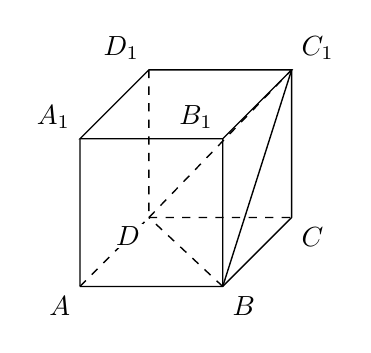
\begin{tikzpicture}[line width=.5pt,scale=1.25]
  \coordinate (A1) at (0,1.7);
  \coordinate (B1) at (1.45,1.7);
  \coordinate (C1) at (2.15,2.4);
  \coordinate (D1) at (.7,2.4);
  \coordinate (A) at (0,.2);
  \coordinate (B) at (1.45,.2);
  \coordinate (C) at (2.15,.9);
  \coordinate (D) at (.7,.9);
  % 上底面、可见外棱与隐藏外棱。
  \draw (A1)--(B1)--(C1)--(D1)--cycle;
  \draw (A1)--(A) (B1)--(B) (C1)--(C) (A)--(B)--(C);
  \draw[dashed] (D1)--(D) (A)--(D) (D)--(C);
  % 截面 BDC_1：BD 位于下底面、DC_1 位于背面，按投影用虚线表示。
  \draw (B)--(C1);
  \draw[dashed] (B)--(D) (D)--(C1);
  \node[above left] at (A1) {$A_1$};
  \node[above left] at (B1) {$B_1$};
  \node[above right] at (C1) {$C_1$};
  \node[above left] at (D1) {$D_1$};
  \node[below left] at (A) {$A$};
  \node[below right] at (B) {$B$};
  \node[below right] at (C) {$C$};
  \node[fill=white,inner sep=1pt,below left=2pt] at (D) {$D$};
\end{tikzpicture}
